\chapter{\label{c:gw-detection}Gravitational waves}

\section{Event GW150914}
Around \num{1.3} billion years ago a pair of black holes, one with \num{36} solar masses and the other with \num{29} solar masses, merged into a single black hole with \num{62} solar masses \cite{Abbott2016}. The missing energy equivalent to \num{3} solar masses was radiated away in the form of gravitational waves.

At 09:50:45 \gls{UTC} on \nth{14} September 2015, gravitational waves from the event passed through the \LIGO{} Livingston detector, perturbing the mirrors by \SI{e-18}{\meter} and creating a signal large enough for the electronics controlling the interferometer to detect the ripple in spacetime more than \num{23} times above the background noise. Seven milliseconds later, the same wavefront passed the \LIGO{} Hanford detector and moved the mirrors in the opposite direction. At that moment, for the first time in human history, a gravitational wave had been detected.

From the gravitational waveform witnessed at the \LIGO{} sites it was possible to determine the type and parameters of the waves' source. The waveforms for \emph{\GWFIRSTEVENT{}}, as it became known, are consistent with a binary black hole merger where they are swept up in frequency before creating a loud ``chirp'' signal as shown in Figure\,\ref{fig:gw150914}. The signal was only above each detector's background noise for the last few \SI{}{\milli\second} of this process. Not only did \LIGO{} make the first observation of a gravitational wave, it also made the first detection of a binary black hole system and found the missing experimental proof of Einstein's theory of general relativity. The window into the universe opening up due to \LIGO{} and the worldwide network of gravitational wave detectors in operation and under assembly, \GEO{}, \VIRGO{} and \KAGRA{}, represents an opportunity to study the universe in a completely new way.

\begin{figure}
  \centering
  \includegraphics[width=\columnwidth]{graphics/generated/from-python/10-gw150914.pdf}
  \caption[Measured strain from the LIGO Hanford and Livingston detectors around the time of event \GWFIRSTEVENT{}]{\label{fig:gw150914}Measured strain from the \LIGO{} Hanford and Livingston detectors around the time of event \GWFIRSTEVENT{}, the first recorded gravitational wave in history. Once a promising signal is identified, a cluster of compute nodes work to find the best fitting waveform from precomputed template banks representing the various combinations of the system's parameters. The waveforms calculated from numerical relativity are shown in the lower panel representing the best fit parameters.}
\end{figure}
% data from https://losc.ligo.org/events/GW150914/

\section{Scientific outcomes from the first joint observation run}
The first detection was made shortly before a science run in which the two \LIGO{} detectors were kept at their most sensitive operating conditions as often as possible for a period of three months. In that time a second detection was made of a separate binary black hole merger, \GWSECONDEVENT{} \cite{Abbott2016b}, and taken alongside the first detection and another signal with lower significance it was possible for the \LSC{} and \VIRGO{} collaboration to make some important scientific discoveries. Among the outcomes from the observation run were that the first experimental tests of strong gravitational fields present during the events were still consistent with general relativity \cite{Abbott2016c}; that ``heavy'' black holes exist in nature and that they probably formed in an environment with low metallicity \cite{Abbott2016d}; and that the rate at which binary black holes merge in the known universe is constrained given the observations to between 9 and 240 per cubic gigaparsec per year \cite{lscvirgoo1}, suggesting that the advanced detectors might see dozens more in subsequent science runs.

Beyond the detection of binary black hole mergers, other sources such as compact neutron star binaries have yet to be found but are predicted to exist with signals within the sensitivity of the detector networks for future science runs \cite{Abbott2016f}. Subsequent observation runs will hope to probe for new sources of gravitational waves, and with longer observations it will be possible to set comprehensive limits on the population of these astrophysical objects in our universe.

The long term goal of researchers in the field is to assemble a worldwide network of gravitational wave detectors to compliment the existing network of electromagnetic (\gls{EM}) telescopes to facilitate \emph{multi-messenger} astronomy. Such a network would be able to localise the sky position incident gravitational waves well enough to allow for \emph{\gls{EM} follow-up} \cite{Abbott2016e, Abbott2016f}, whereby the data from both telescopes and gravitational wave detectors could be combined to probe the astrophysics of the events in unprecedented detail and to identify and learn more about the nature and origin of host galaxies.

\section{General relativity and gravitational waves}
A consequence of Einstein's theory of general relativity, gravitational waves are produced by changes in the quadrupole moment of a distribution of mass. The effect a gravitational wave has on spacetime is to stretch it in one direction while contracting it in another. This \emph{strain} can be expressed as a linear combination of ``plus'' and ``cross'' polarisation terms, shown for an initially circular ring of test particles as a function of phase angle in Figure\,\ref{fig:gravitational-wave-polarisation}.

\begin{figure}
  \centering
  \includegraphics[width=\columnwidth]{graphics/generated/from-svg/10-gravitational-wave-polarisation.pdf}
  \caption[Plus and cross polarisations of a propagating gravitational wave]{\label{fig:gravitational-wave-polarisation}Plus and cross polarisations of a propagating gravitational wave. As the wave travels, it stretches spacetime in one direction while contracting it in the other in an elliptic behaviour. A gravitational wave's propagation can be described as a linear combination of the two polarisations.}
\end{figure}

Gravitational waves from Earth-bound mass distributions, including the Earth itself, are not even remotely detectable. The strain in spacetime produced by such objects is so weak that there is no hope for us to make such a detection with any known technology. A good estimate for the strain produced by a pair of rotating objects is given in \cite{Sathyaprakash2009} as:
\begin{equation}
  \label{eq:happrox}
  h \lesssim \frac{2 G \left( M v^{2} \right)_{\text{nonspherical}}}{c^4 r},
\end{equation}
where $G$ is the gravitational constant, $\left( M v^{2} \right)_{\text{nonspherical}}$ is the kinetic energy associated with the non-spherical parts of the source, $c$ is the speed of light and $r$ is the distance to the source. To get an idea of what the spacetime strain would be for man-made sources, we can consider as in \cite{Sathyaprakash2009} the case of two cars of mass $M = \SI{e3}{\kilo\gram}$ attached to opposite ends of a rod of length $d = \SI{10}{\meter}$, spinning about its centre in a centrifuge at a frequency of $f = \SI{10}{\hertz}$. The tangential velocity of the cars will be around $2 \pi f d \approx \SI{600}{\meter\per\second}$. Placing the detector one wavelength away, and using Equation\,\ref{eq:happrox}, the strain turns out to be around $\SI{4e-43}{}$. To be able to detect such a strain the current most sensitive detectors, \ALIGO{}, would require an improvement in sensitivity of \SI{20}{} orders of magnitude, which is clearly ludicrous.

A pair of solar-mass objects orbiting each other at \SI{100}{\hertz} within \SI{50}{\mega\lightyear} produces a strain of only one part in \SI{e21}{}, which is a strain only now detectable after decades of detector development, and a feat once thought impossible in the early \nth{20} Century. It is only the waves produced by the most massive objects in the universe which we have any chance of detecting: black holes, compact binary neutron stars and supernovae amongst others. Even then, gravitational radiation is only produced by the presence of a changing quadrupole moment, and so only a subset of sources that happen to be in coalescence or contain surface asymmetries produce waves we have the ability to detect.

\section{Development of the gravitational wave detector}
Using the \emph{local Lorenz} gauge an incident gravitational wave can be described as a change in length between two test masses. The primary degree of freedom a gravitational wave excites is the differential mode of the space separating the test masses, \LMINUS{}, which can be defined in terms of the position of the test masses $x_{\textrm{A}}$ and $x_{\textrm{B}}$ as:
\begin{equation}
  \label{eq:darm}
  \textrm{\LMINUS{}} = \frac{x_{\textrm{A}} - x_{\textrm{B}}}{2}.
\end{equation}
The strain of an incident gravitational wave can be determined from this change in length.

The first attempts to detect gravitational waves began with Joseph Weber's studies in the 1960s with his \emph{Weber bar} \cite{Weber1960}. This was a device developed to act as a direct strain meter, with incident gravitational waves exciting modes between the two ends of the bar effectively forming the test masses. Piezoelectric sensors placed on the surface of an aluminium cylinder convert changes in length into electrical signals. Whilst the expected change in length of such a cylinder from gravitational radiation would in most cases be tiny, the resonant frequency of the cylinder, typically in the kilohertz range, acts to enhance the amplitude of the length change at nearby frequencies. The sensitivity of such a bar as a function of frequency is determined in part by its quality factor (Q), with a necessary trade-off being made between peak sensitivity (high Q) and detection bandwidth (low Q). As sources of gravitational radiation are almost universally weak, the only reasonable hope of making such a detection is to choose a high Q material and hope for a favourable signal frequency.

The original resonant bar detectors were evolved over time to become cryogenic, to decrease the effect of thermal noise; and spherical, to maximise the test mass's Q. Despite such improvements the peak sensitivity of state-of-the-art resonant bar detectors was surpassed by \emph{interferometric} gravitational wave detectors in 2003 \cite{Pitkin2011} after it was shown that \emph{second generation} detectors improving upon the initial designs would offer superior sensitivity across a much wider bandwidth \cite{Harry2002a}. The interferometer was first suggested as a means for gravitational wave detection shortly after the introduction of the Weber bar\footnote{The first known example being by Gertsenshtein and Pustovoit in the Soviet \emph{Journal of Experimental and Theoretical Physics} in 1962.}, but efforts to build prototypes and understand the significant sources of noise only gained momentum in the 1970s \cite{Moss1971, Weiss1972}.

\subsection{\label{sec:gw-interferometry}The gravitational wave interferometer}

% keep this here - it's referenced throughout this section
\begin{figure}
  \begin{center}
    \begin{subfigure}{.3\textwidth}
      \includegraphics[width=\columnwidth]{graphics/generated/from-svg/10-michelson.pdf}
      \caption{Simple \MI{}}
      \label{fig:mi}
    \end{subfigure}
    \hfill
    \begin{subfigure}{.3\textwidth}
      \includegraphics[width=\columnwidth]{graphics/generated/from-svg/10-fabry-perot-michelson.pdf}
      \caption{\FPMI{}}
      \label{fig:fpmi}
    \end{subfigure}
    \hfill
    \begin{subfigure}{.3\textwidth}
      \includegraphics[width=\columnwidth]{graphics/generated/from-svg/10-dual-recycled-fabry-perot-michelson.pdf}
      \caption{\DRFPMI{}}
      \label{fig:drfpmi}
    \end{subfigure}
    \caption[The evolution of the gravitational wave detector]{The evolution of the gravitational wave detector. Figure\,\ref{fig:mi} shows the simple \MI{} used since the famous Michelson and Morley experiments of the 1880s, and proposed for gravitational wave detection in early literature. Figure\,\ref{fig:fpmi} shows a \MI{} with the addition of \FP{} arm cavities to enhance sensitivity. Figure\,\ref{fig:drfpmi} shows a \FPMI{} with the addition of recycling mirrors.}
  \end{center}
\end{figure}

Figure\,\ref{fig:mi} shows the \MI{} topology that all current detectors are based on. Gravitational waves modulate the phase of the interferometer light in the arms, and the amount of modulation depends on the ratio of the light's frequency $f_0$ and the gravitational wave frequency $f_g$. A \MI{} can be made by taking coherent light from a laser, splitting it into two parts then shining one on a mirror. Comparing the phase of the reflected light field to the other light field it is possible to detect passing gravitational waves by an additional phase accumulation on the returning light on top of the expected round trip phase with respect to the first. The change in the arm length $\Delta L$ with respect to the nominal length $L$, which gives the gravitational wave's \emph{strain}, is then given by:
\begin{equation}
  \label{eq:freq-to-length}
  \frac{\Delta L}{L} = \frac{\Delta f}{f},
\end{equation}
where $\Delta f$ is the measured change in laser frequency at the detector normalised by the carrier frequency $f$. Gravitational wave induced phase modulation can also be described with the \emph{transverse traceless} gauge as a change in the refractive index of the light between the test masses. The effect is equivalent.

The simple \MI{} design has a number of disadvantages. Using the standard ground-based gravitational wave detector wavelength ($\lambda_0 = \SI{1064}{\nano\meter}$), when the arm length is optimal for a gravitational wave of frequency $\SI{e3}{\hertz}$, the wave's phase modulation effect on the light is of the order $\frac{f_0}{f_g} = \frac{\SI{e14}{}}{\SI{e3}{}} = \SI{e11}{}$ which gives an estimate of the strain enhancement in the interferometer. Gravitational radiation from likely sources reaches us with strain of at most \SI{e-21}{} meaning that the interferometer's electronics would need to be capable of making a phase measurement of at least \SI{e-10}{\radian}: a very difficult feat. Furthermore, the optimal antenna length for a gravitational wave detector is $\frac{c_0}{4 f_g}$ \cite{Abbott2016a}, as with electromagnetic antennae, and so for this frequency the arm would ideally be \SI{75}{\kilo\meter}. This is clearly impractical for ground based detectors.
% from http://imprs-gw.aei.mpg.de/miscellaneous/05_downloads/imprs-lecture-weeks/march-2014/experimental-gw-physics/modulation/

\subsubsection{\label{sec:fabry-perot-cavities}\FP{} arm cavities}
One way to simultaneously reduce the phase measurement requirement and the effective arm length is to use \FP{} cavities\footnote{Other techniques were tested around this time such as delay lines, though they were found to have additional technical challenges for no greater benefit \note{cite something from Garching?}.}. \FP{} cavities increase a photon's effective path length by reflecting it many times between two partially transmitting mirrors. While this improves on the \MI{}'s phase measurement requirement by approximately the cavity gain (a function of the mirror reflectivities, typically of the order \num{100} to \num{1000}), this still leaves the interferometer susceptible to fluctuations in the laser's frequency which are indistinguishable from signal. This problem can be addressed through the use of \FP{} cavities in the arms of a \MI{}. By placing two arm cavities at the reflected and transmitted ports of the beam splitter the light that recombines at the output port contains out-of-phase copies of the laser's frequency fluctuations which cancel out. A \emph{\FPMI{}} is shown in Figure\,\ref{fig:fpmi}.

\subsubsection{\label{sec:power-recycling}Power recycling}
The \FPMI{} can provide good cancellation of laser frequency noise and good sensitivity to differential arm length fluctuations, but one problem is still apparent: the vast majority of the light that recombines at the beam splitter is sent back towards the laser, where it samples the position of input optics not necessarily isolated from the ground and interferes with the laser crystal. This light is typically rejected by means of a Faraday isolator, leading to power loss. To save this light from being lost, an additional mirror can be placed at the input to reflect the light returning to the laser back into the interferometer. This technique is called \emph{power recycling}, and it increases the power in the arms by approximately the gain of the cavity the power recycling mirror forms with each arm's input mirrors. The \emph{first generation} \ILIGO{}, \IVIRGO{} and \IVIRGO{} detectors were \PRFPMI{}s.

\subsubsection{\label{sec:signal-recycling}Signal recycling}
Signal recycling is an evolution on the \PRFPMI{}, which involves the placement of a \emph{signal recycling} mirror at the output port of the interferometer, whereby the signal created at the output of the interferometer can be enhanced in a certain frequency band by the creation of an additional \emph{signal recycling cavity} \cite{Meers1988}. The signal recycling mirror's transmissivity and position can be modified to determine the frequency range over which this enhancement occurs due to the dynamics of the cavity \cite{Buonanno2001}.

\subsubsection{Dual recycling with \FP{} arm cavities}
The natural combination of power and signal recycling with the \FPMI{} leads to the \emph{\DRFPMI{}} shown in Figure\,\ref{fig:drfpmi}. This is the topology that provides the greatest sensitivity, either broadband or narrowband depending on the tuning of the signal recycling cavity, for a given laser power, arm length and mirror mass; it is therefore the topology employed in current generation detectors. The use of \emph{dual recycling} was initially demonstrated in both table-top and suspended prototype experiments \cite{Strain1991, Heinzel1998, Freise2000}, and later a full-scale dual-recycled \MI{} detector was demonstrated at \GEO{} \cite{Heinzel2002, Grote2004}. The \ALIGO{} detectors were the first to fully implement the \DRFPMI{} topology.

\section{Current and future detectors}
As of the time of writing the \ALIGO{} detectors are online and commissioners are working towards reaching the design sensitivity. \AVIRGO{} is due to begin science operations towards the end of 2016, with \KAGRA{} due to follow in 2019. \GEOHF{} has been operational in the years since the initial detectors stopped for upgrades, and is now transitioning into a detector-scale prototype facility. Planning is also under way to build an \ALIGO{} detector in India. The eventual network of detectors is shown in Figure\,\ref{fig:detector-network}.

Beyond this generation, plans are afoot to build facilities which will push the sensitivity of the gravitational wave detector to the limit, with the so-called \emph{third generation} detectors. A European collaboration is working towards the \emph{\ET{}} \cite{ET2011} and the \LSC{} is working towards \emph{\LIGOCE{}} \cite{Dwyer2015}. Efforts are also under way to complement the ground-based detectors with a space-based counterpart with significantly enhanced low frequency sensitivity, \emph{\ELISA{}} \cite{Amaro-Seoane2012}. Together, the network of ground- and space-based detectors will provide unprecedented sensitivity from frequencies of \SI{}{\milli\hertz} to \SI{}{\kilo\hertz}, presenting the ability to study the universe in unparalleled fidelity.

\begin{figure}
  \centering
  \includegraphics[width=\textwidth]{graphics/generated/from-python/10-detector-network.pdf}
  \caption[Worldwide detector network]{\label{fig:detector-network}Worldwide detector network. \GEO{}, \LHO{} and \LLO{} are operational, whilst \VIRGO{} and \KAGRA{} are being commissioned and \INDIGO{} is under construction. The locations of the \ET{} and \LIGOCE{} are as yet undecided.}
\end{figure}

\section{Thesis structure}
This thesis outlines work conducted with the goal of improving the sensitivity of future gravitational wave observatories.

Chapter\,\ref{c:instrumentation} introduces some theoretical foundations and motivation for the work presented in the rest of this thesis. Chapter\,\ref{c:waveguides} presents an investigation into \emph{waveguide} mirrors which offer a large potential improvement in Brownian thermal noise over conventional dielectric mirrors. One downside is the potential presence of a coupling effect between transverse motion and reflection phase. This chapter presents an experiment conducted to measure this coupling in order to give a clearer picture of this type of mirror's potential use in future gravitational wave facilities.

The next set of chapters, \ref{c:speedmeter-intro}, \ref{c:speedmeter-control} and \ref{c:esd-concept}, present experimental research into a new type of gravitational wave interferometer: the \SSM{}. Chapter\,\ref{c:speedmeter-intro} introduces the concept in more detail and presents an overview of an ongoing proof-of-principle experiment taking place in Glasgow. Chapter\,\ref{c:speedmeter-control} highlights an important technical problem with the \SSM{} configuration which is not present with current detectors: that the controller cannot determine the displacement of the cavity mirrors at low frequencies, leading to loss of sensitivity. A solution to the problem is presented through the modelling of the complete control system using existing measurements of the response and noise of the apparatus as well as estimates for noise in the experiment as fully assembled, backed by numerical simulations. Finally, Chapter\,\ref{c:esd-concept} outlines the architecture and construction of experimental apparatus to test a new actuator design to be used in the \SSMEXPT{}: a plate capacitor electrostatic actuator. Designs and tests of high-voltage equipment to create the required test mass actuation are presented \note{along with some preliminary results}.

The main body of the work concludes with Chapter\,\ref{c:et-lf-control} where the current state of the sensing and control design for the low frequency interferometer as part of the planned Einstein Telescope facility is presented. This interferometer is to be primarily sensitive to frequencies below \SI{10}{\hertz} where existing detectors are dominated by seismic noise. Here, the state of the art sensing, controls and actuators found in the current generation of detectors are revisited through the use of numerical simulations.

Finally, the appendices provide additional information for the enthusiastic reader to support the main work. Appendix\,\ref{a:interferometry} provides a mathematical description of a basic interferometer and derives some useful figures of merit used throughout the work to describe interferometers. Appendix\,\ref{a:simulation-tools} discusses the differences between the two main numerical simulation tools used for the presented work in Chapters \ref{c:speedmeter-intro}, \ref{c:speedmeter-control} and \ref{c:et-lf-control}. A conclusion is provided in Chapter\,\ref{c:conclusion}.